\documentclass[notes]{beamer}
\usetheme{Madrid}
\usepackage[utf8]{inputenc}
\usepackage{amsmath}
\usepackage{amsfonts}
\usepackage{amssymb}
\newcounter{saveenumi}
\newcommand{\seti}{\setcounter{saveenumi}{\value{enumi}}}
\newcommand{\conti}{\setcounter{enumi}{\value{saveenumi}}}

\resetcounteronoverlays{saveenumi}
%\author{}

\usepackage{geometry} 
\usepackage{array}
\usepackage{float}
\usepackage{placeins}
\usepackage{xcolor}
\usepackage{cancel}
\usepackage{graphicx}
\usepackage{tikz} 
\usepackage[overlay]{textpos}
\usepackage{hyperref}
\usepackage{animate}
\usepackage{wasysym}
\usepackage{listings}

 
 
\newcommand{\tikzmarkk}[2][minimum width=6cm,minimum height=1.5cm]{
 \tikz[remember picture,overlay]
 \node[anchor=west,
       inner sep=0pt,
       outer sep=6pt,
       xshift=-0.5em,
       yshift=-3ex,
       #1](#2){};
}

\newcommand{\shownode}[1]{
  \tikz[remember picture,overlay]\draw[red](#1.south east)rectangle(#1.north west);
}

\newcommand{\showanchor}[1]{
  \tikz[remember picture,overlay]\draw[red,thick,mark=x] plot coordinates{(#1)};
}

% original code from Stefan Kottwitz
% http://tex.stackexchange.com/a/12551/13304
\newenvironment<>{varblock}[2][.9\textwidth]{%
  \setlength{\textwidth}{#1}
  \begin{actionenv}#3%
    \def\insertblocktitle{#2}%
    \par%    
    \usebeamertemplate{block begin}%
    }
  {\par%
    \usebeamertemplate{block end}%
  \end{actionenv}}

\newenvironment{myblock}[1]{\begin{textblock*}{500pt}(#1)}{\end{textblock*}}

% special way to reach the top of the block
\def\newabove(#1){
([yshift=1.5ex]#1.center)
}

\definecolor{dgreen}{rgb}{0.,0.6,0.}
\colorlet{dgr}{green!70!black}
\definecolor{aqua}{rgb}{0.0, 0.2, 1.0}

 
\definecolor{persianindigo}{rgb}{0.2, 0.2, 0.7}  
\newcommand{\indigo}[1]{\textcolor{persianindigo}{#1}}

\definecolor{red}{rgb}{1.0, 0.0, 0.0}  
\newcommand{\red}[1]{\textcolor{red}{#1}}

\title{MicMac V1/V2 état d'avancement}
\subtitle{\textcolor{lightgray}{Ajustement de faisceaux}}
\author{Marc Pierrot Deseilligny 
%\footnotesize \textit{with support slides from A Pinte and M Pierrot Deseilligny}
} 

\institute
{
	Univ. Gustave Eiffel -- IGN/ENSG, LaSTIG lab.- France 
}

\date{novembre 2022}

\graphicspath{{./img/}}

%vertical curmy braces 
\usetikzlibrary{decorations.pathreplacing,calc}
\newcommand{\tikzmark}[1]{\tikz[overlay,remember picture] \node (#1) {};}
  
\begin{document}


%%%%%%%%%%%%%%%%%%%%%%%%%%%%%%%%%%%%%%%%%%%%%%%%%%%%%%
\begin{frame}
\section{Ajustement de faisceaux}

\begin{center}
{\bf {\Large Ajustement de faisceaux}}
\end{center}

\end{frame}
%%%%%%%%%%%%%%%%%%%%%%%%%%%%%%%%%%%%%%%%%%%%%%%%%%%%%%

  %   -  -  -  -  -  -  -  -  -  -  -  -  -  -  -  -  -  -  -  -  -  -  -  -
\begin{frame}{Equation de projection}

Equation "principale", de projection classique  avec les notations ;

\begin{enumerate}
    \item  le point  terrain  $P_j$ visible and $k$
    \item  le senseur  $k$ avec une fonction de projection terrain-image $\pi_k$;
    \item  le point  image  $q_{j,k}$ visible and $k$
\end{enumerate}

Pour tous les point où  $P_j$ est visible dans $\pi_k$ :

\begin{equation}
    \pi_k (P_j) = q_{j,k} \label{EqPrinc}
\end{equation}

Ici $\pi_k$  est inconnu, $q_{j,k}$ est une observation et $P_j$  peut être suivant les cas :

\begin{enumerate}
    \item  une observation ;
    \item  une inconnue avec des observations;
    \item  une inconnue sans obervation (point de liaison multiple ou non).
\end{enumerate}


\end{frame}

  %   -  -  -  -  -  -  -  -  -  -  -  -  -  -  -  -  -  -  -  -  -  -  -  -

\begin{frame}{Formalisation}

En plus de l'équation "principale" \ref{EqPrinc}, on un certain nombre d'équation auxiliaires
.(bloc, GPS \dots) non détaillées ici $A_i$.  Comme on a (beaucoup) plus d'inconnues que d'équations ,
on formalise le problème par moindre carrés :

\begin{equation}
    \sum_{j,k}  |\pi_k (P_j) - q_{j,k} |^2  + \sum_i A_i^2  \label{EqLstSq}
\end{equation}

Comme le système n'est pas linéaire on le linéarise par différenciation. 

Comme la linérisation est une approximation on itère.

\end{frame}

  %   -  -  -  -  -  -  -  -  -  -  -  -  -  -  -  -  -  -  -  -  -  -  -  -

\begin{frame}{Implementation}

Le diable est dans les détails \dots Il reste à définir notamment :

\begin{enumerate}

   \item comment calculer les dérivées;

   \item comment stocker  les systèmes de moindres carrés;

   \item comment gérer les grands systèmes avec des $10^4 \dots 10^6$ points de liaisons;

   \item comment résoudre les systèmes de moindres carrés;

   \item quel modèles de caméra;
\end{enumerate}

\end{frame}

  %   -  -  -  -  -  -  -  -  -  -  -  -  -  -  -  -  -  -  -  -  -  -  -  -

\begin{frame}{Calcul des dérivées-1}

Les principales méthodes de calcul des dérivées sont :

\begin{enumerate}
    \item à la main  ; $+$ efficace ,  $-$ source d'erreur, difficile à maintenir; 

    \item  dérivées numérique  ; $+$ simple, $-$ lent, risque d'imprécision;

    \item  jet  : $+$ exact  , $-$ un peu lent , un peu compliqué à développer 
           (NB un jet = 1 nombre + un infiniment petit formel, voir  CERES)

    \item   dérivées symboliques : $+$ exact et rapide , $-$ moyennement compliqué à développer (mais assez simple à utiliser)

    \item   code differenciation : $+$ exact et rapide, permet de dériver des expression avec des boucles 
            $-$ très compliqué à développer et assez compliqué à utiliser.
\end{enumerate}

La méthode utilisée dans MicMac  (V1 et V2) est celle des dérivées symboliques.

\end{frame}

  %   -  -  -  -  -  -  -  -  -  -  -  -  -  -  -  -  -  -  -  -  -  -  -  -

\begin{frame}{Calcul des dérivées-2}

Représentation des formules comme un arbre :

\begin{figure}
   \centering
	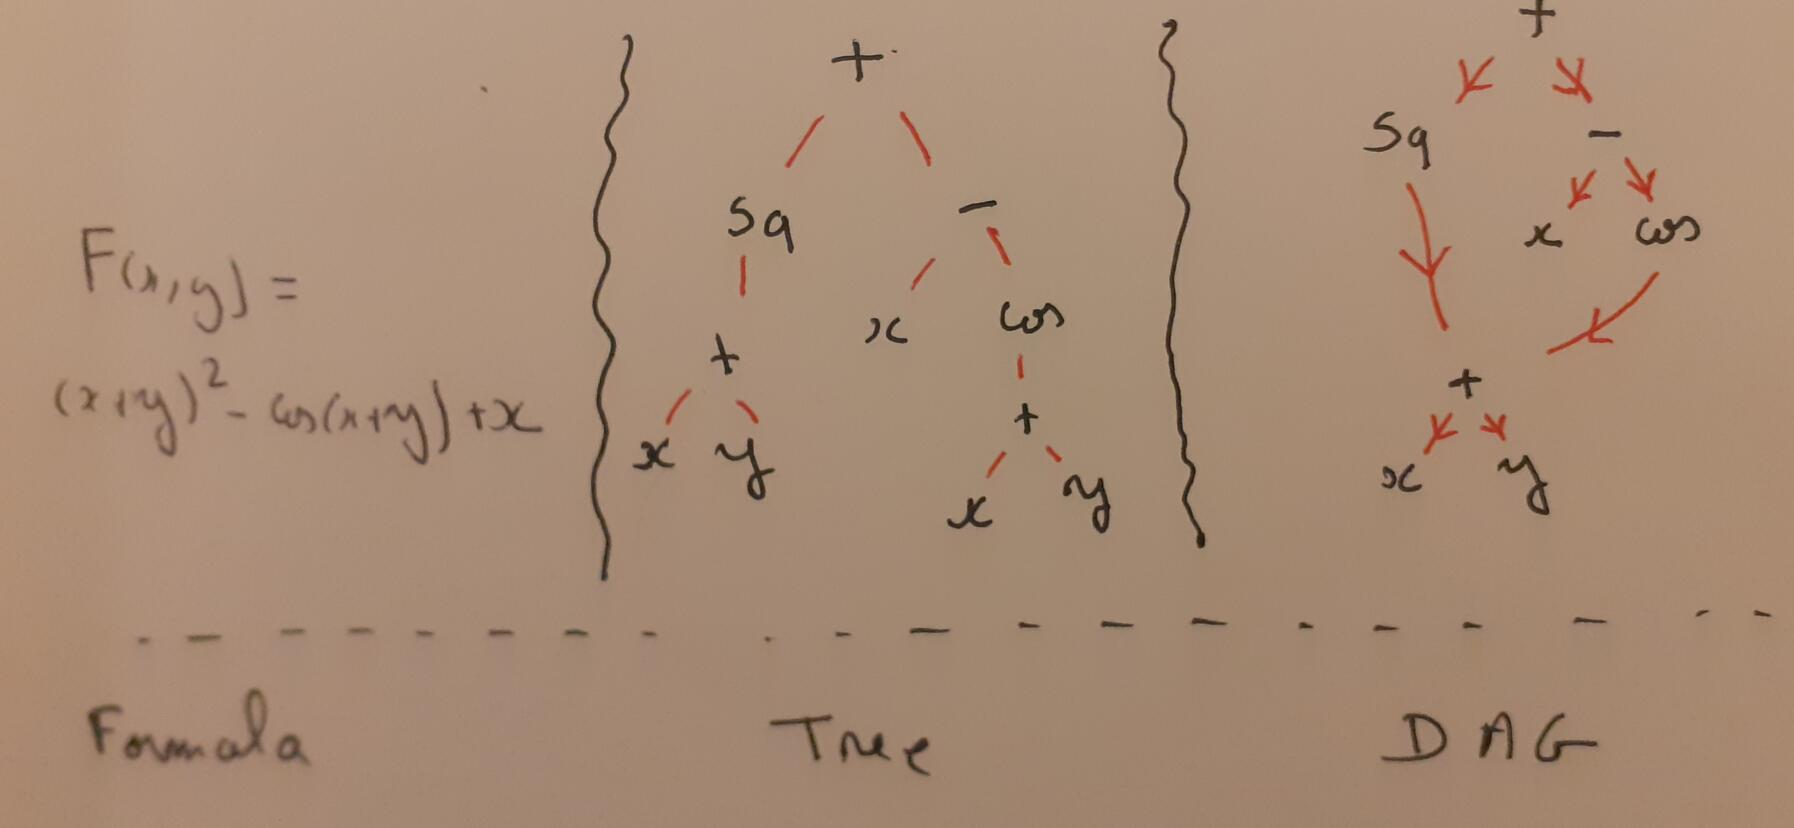
\includegraphics[width=0.5\textwidth]{../Programmer/ImagesProg/Tree.jpg}
   \label{fig:chambre_noire_pic}
\end{figure}

On définit toute les opérations sur les arbres de formules.

\end{frame}

  %   -  -  -  -  -  -  -  -  -  -  -  -  -  -  -  -  -  -  -  -  -  -  -  -

\begin{frame}[fragile]{Calcul des dérivées-3}

{\tiny

\begin{lstlisting}[language=c++]

begin{lstlisting}[language=c++]
// === Extract of code in class cMulF (multiplication of formulas )

// method for computing values
void ComputeBuf(int aK0,int aK1) override
{
    for (int aK=aK0 ; aK<aK1 ; aK++)
        mDataBuf[aK] =  mDataF1[aK] * mDataF2[aK];
}

// method for computing the derivative
cFormula<TypeElem> Derivate(int aK) const override
{
   return  mF2*mF1->Derivate(aK) + mF1*mF2->Derivate(aK);
}

// method for generating the code
std::string GenCodeDef() const override
{
    return "(" + mF1->GenCodeRef() + " " + this->NameOperator() +  " " + mF2->GenCodeRef() + ")";
}
\end{lstlisting}

}

\end{frame}

  %   -  -  -  -  -  -  -  -  -  -  -  -  -  -  -  -  -  -  -  -  -  -  -  -

\begin{frame}{Calcul des dérivées-4}

Les formules identiques sont identifiées, le code est représenté comme un DAG :

\begin{figure}
   \centering
	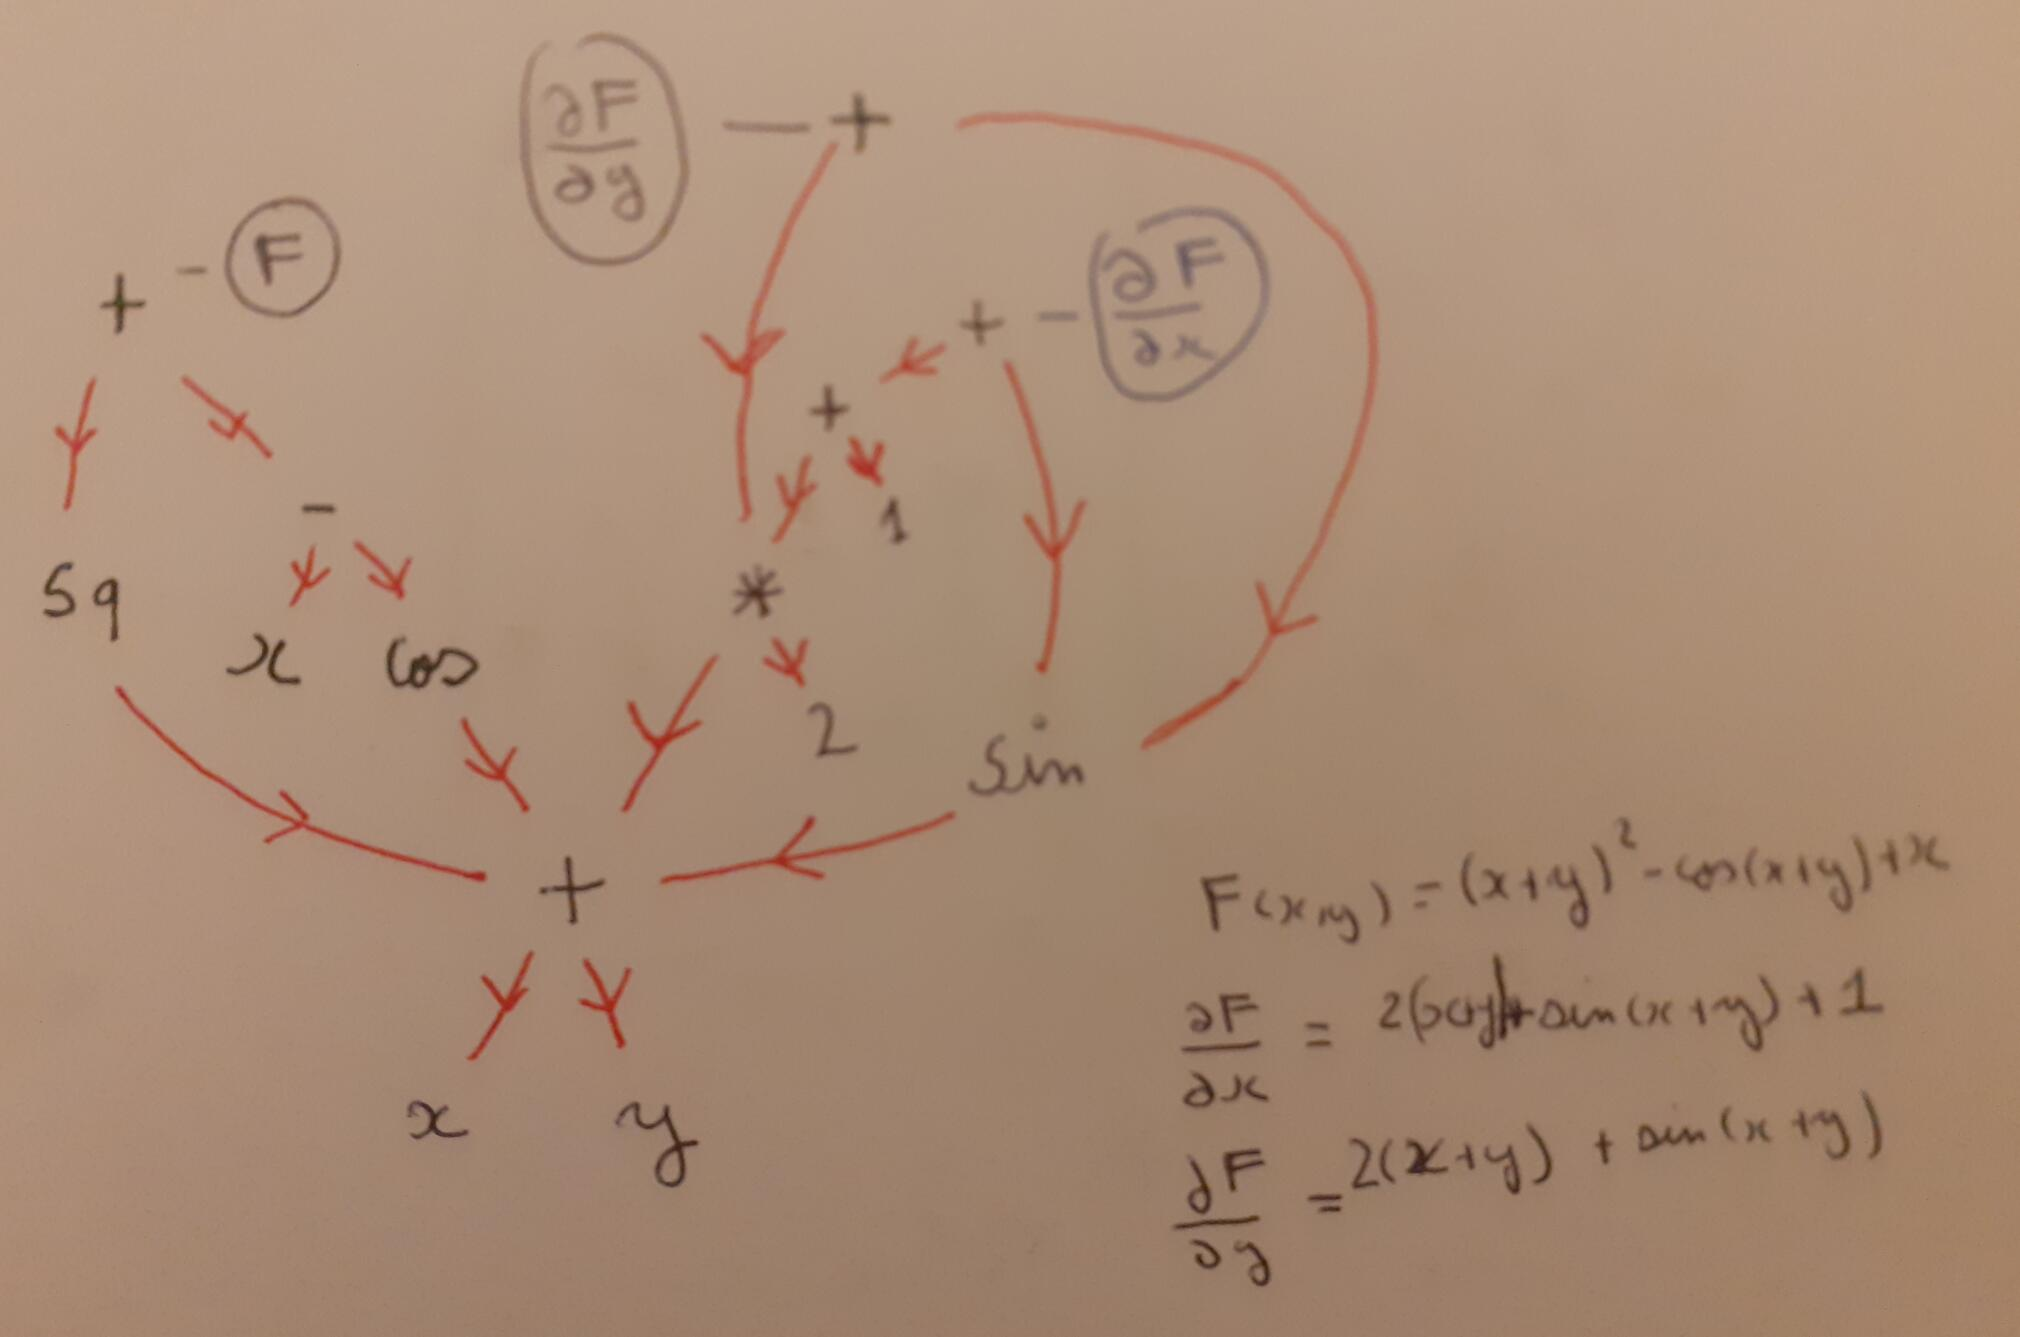
\includegraphics[width=0.5\textwidth]{../Programmer/ImagesProg/DAG.jpg}
   \label{fig:chambre_noire_pic}
\end{figure}


\end{frame}

  %   -  -  -  -  -  -  -  -  -  -  -  -  -  -  -  -  -  -  -  -  -  -  -  -

\begin{frame}{Calcul des dérivées-5}

{\tiny 
Les principales règles de réductions sont utilisées :

\begin{itemize}
     \item  $0*F \rightarrow 0$ ,   $1*F  \rightarrow F$ , $-1*F \rightarrow -F$ (and idem $F*0\dots$);

     \item  $0/F \rightarrow 0$ ;

     \item  $0+F \rightarrow F$ ,   (and idem $F+0\dots$);

     \item  $-(-F) \rightarrow F$ ,  $F_1-(-F_2) \rightarrow F_1+F_2$;

     \item  $F_1*F_2 + F_1*F_3  \rightarrow F_1*(F_2+F_3)$ , $F_1*F_2 - F_1*F_3  \rightarrow F_1*(F_2-F_3)$ ,
     \item  $F_2/F_1 + F_3/F_1  \rightarrow (F_2+F_3)/F1$ ,  $F_2/F_1 - F_3/F_1  \rightarrow (F_2-F_3)/F1$ ,

     \item if  $F_1 > F_2$ then  $F_1 + F_2  \rightarrow F_2 + F_1$ , here the comparison $F_1 > F_2$
           is made on numbering, this rules is here favorize merging in DAG creation , any comparison as long
           as it anti-symetric would hold; we just want to avoid that in the same formula $F_1+F_2$ and $F_2+F_1$
           cannot be merged;
     \item if  $F_1 > F_2$ then  $F_1 * F_2  \rightarrow F_2 * F_1$

     \item  $C(a) \otimes C(b) \rightarrow C(a \otimes b) $  where  $C(x)$ design the formula for constant $x$
             and $\otimes$ is any bynary operator;
     \item  $ \alpha (C(a)) \rightarrow C(\alpha (a)) $  where  $\alpha$ design any unary operator;

\end{itemize}

}

\end{frame}

  %   -  -  -  -  -  -  -  -  -  -  -  -  -  -  -  -  -  -  -  -  -  -  -  -

\begin{frame}{Calcul des dérivées-6}
Le code généré ressemble à quelques chose comme cela :

\vline

{\small
{\tt
    double F29 = std::sin(F8);

    double F13 = MMVII::DerSinC(F8);

    double F14 = (2 * F8);

    double F9 = MMVII::sinC(F8);

    double F16 = (F15 / F14);

    double F10 = (F9 * PixI);

    double F22 = (F21 / F14);

    double F11 = (F9 * PixJ);

    double F18 = (F16 * F13);

    double F32 = -(F22);

    double F24 = (F22 * F13);
}
}


\end{frame}

  %   -  -  -  -  -  -  -  -  -  -  -  -  -  -  -  -  -  -  -  -  -  -  -  -

\begin{frame}{Modélisation des caméras, cas spatial-1}

Pas encore fait dans V2, mais on compte reprendre en partie le même principe que dans V1:


\begin{enumerate}
    \item hypothèse : la position est précise (GPS sans obstruction), l'imprécision vient de l'orientation;
    \item la  correction est une déformation image  lisse, indépendante du relief;
\end{enumerate}

Modèle de projection :

\begin{equation}
   \pi  =  D \circ \pi_0
\end{equation}
On se donne pour $D$ un modèle paramétrique de type polynomial en $x,y$. 
\end{frame}

  %   -  -  -  -  -  -  -  -  -  -  -  -  -  -  -  -  -  -  -  -  -  -  -  -
\begin{frame}{Modélisation des caméras, cas spatial-1}
Eventuellement on le contraint localement à être proche
des rotations , avec $O,P,K $ trois fonctions de $x$ à variation lente.

\begin{equation}
   D  (x,y)  \approx O(x)  \frac {\partial \pi_0} {\partial \omega} + P(x) \frac {\partial \pi_0} {\partial \phi} + K(x)\frac {\partial \pi_0} {\partial \kappa}
   \label{WPK}
\end{equation}

En pratique dans la majorité des chantier traités en recherche (emprise limitée) on se limite au degré 1 en $x,y$ et on n'utilise peu~\ref{WPK}.
Cette formalisation serait probablement à revoir dans le cadre d'un usage IGN sur de longues bandes.

\end{frame}




\end{document}
